% \chapter{Понятие системы электронного документооборота} \label{chapt1}
\subsection{Общая схема электронного документооборота} \label{doc_scheme}
% \addcontentsline{toc}{chapter}{Понятие системы электронного документооборота}  % Добавляем его в оглавление

% \textbf{\textit{Документооборот}} -- движение документов в организации с момента их создания или получения до завершения исполнения или отправления.\cite{bib1}


\begin{figure} [h] 
  \center
  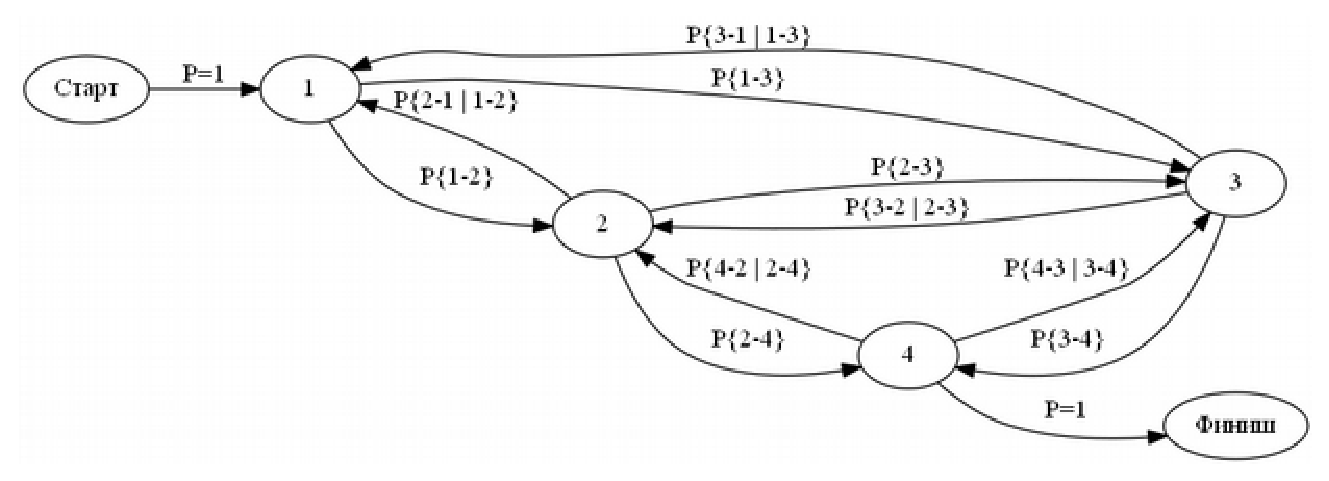
\includegraphics [scale=0.7] {graph1}
  \caption{Характерный вид процесса документооборота} 
  \label{img:graph1}  
\end{figure}


Процесс документооборота можно представить в виде графа, изображённого на рис. \ref{img:graph1}. Вершинами в нём являются редакторы, а дугами -- переходы задания на разработку документа между редакторами в соответствии с принятой в организации структурой. Весам дуг соответствуют вероятности этих переходов. Обратные связи демонстрируют возвращение документа на переработку. Вершинами «Старт» и «Финиш» обозначены момент получения задания и завершение исполнения соответственно.

\vspace{\baselineskip}
В ходе практики была рассмотрена система электронного документооборота.

\vspace{\baselineskip}
\textbf{\textit{Электронный документ}} -- документированная информация, представленная в электронной форме, то есть в виде, пригодном для восприятия человеком с использованием электронных вычислительных машин, а также для передачи по информационно-телекоммуникационным сетям или обработки в информационных системах.\cite{bib2}

\vspace{\baselineskip}
\textbf{\textit{Система электронного документооборота (СЭД)}} -- автоматизированная система, реализующая процесс документооборота применительно к электронным документам.

\vspace{\baselineskip}
Для организации системы электронного документооборота необходимо разработать ряд технических средств, среди которых хранилище электронных документов (ХЭД). В настоящее время электронный архив (одно из распространённых названий ХЭД) позиционируется как независимый компонент, способный быть как отдельным комплексом, заменяющим собой бумажный архив документов, так и основой для СЭД. Данный подход позволяет конструировать гибкую систему электронного документооборота из независимых модулей.

\vspace{\baselineskip}
При проектировании ХЭД следует учитывать законодательно-нормативные требования, касающиеся информационной безопасности хранимых электронных документов. Это обстоятельство позволяет конкретизировать определение ХЭД как \textbf{конфиденциальное хранилище электронных документов (КХЭД)} – систему кратковременного и долговременного конфиденциального хранения электронных документов, предоставляющую возможности по защите от несанкционированного доступа (НСД), контролю доступа, обеспечению юридической значимости электронных документов. \cite{bib3}

\vspace{\baselineskip}
Сложная структура, многоэтапное обслуживание, случайный характер моментов поступления запросов пользователей и длительности их обработки в КХЭД предопределяют использование моделей сетей массового обслуживания для анализа и проектирования.


% \subsection{Структура КХЭД} \label{sect1_2}

% На рис. \ref{img:uml} изображена схема описанных модулей в нотациях UML.

% % \begin{figure} [h] 
% %   \center
% %   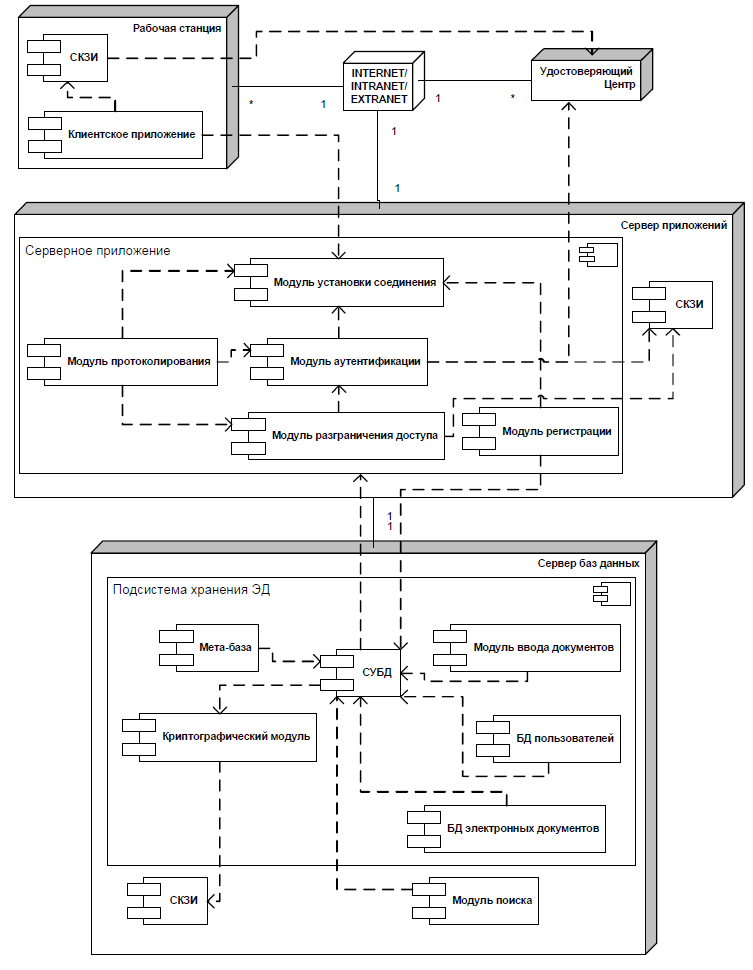
\includegraphics [scale=0.6] {uml.png}
% %   \caption{Структура КХЭД} 
% %   \label{img:uml}  
% % \end{figure}
% \begin{figure}[p]
%   \centering
%   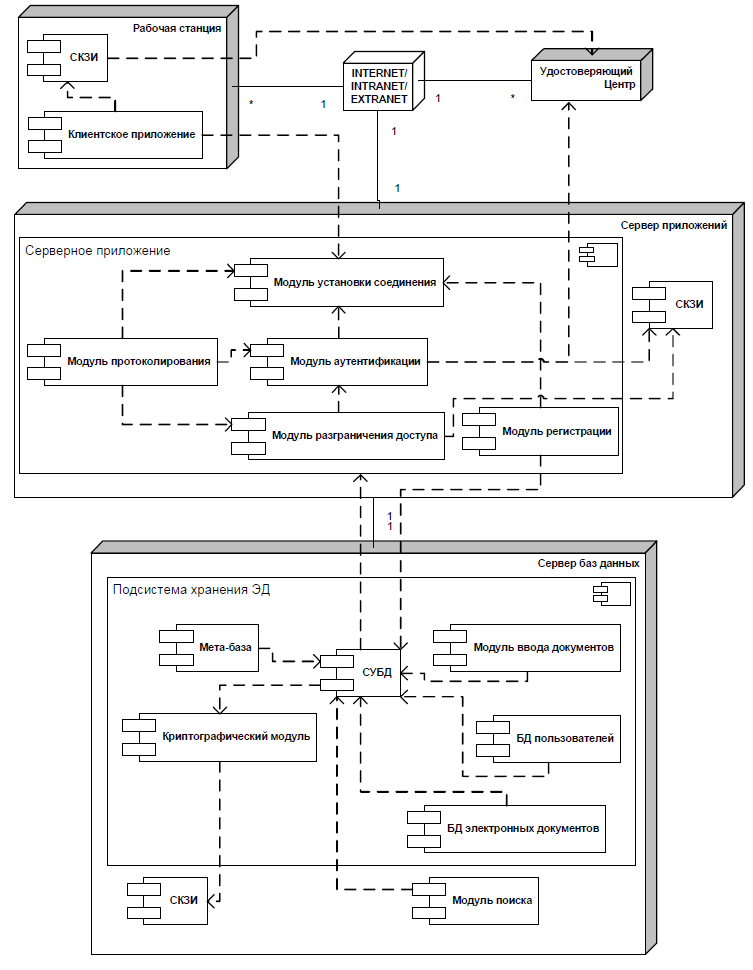
\includegraphics[width=1\textwidth]{uml}
%   \caption{Структура КХЭД}
%   \label{img:uml}
% \end{figure}

% \subsection{Модуль установки соединения} \label{subsect1_2_1}

% Отвечает за организацию процесса подключения пользователя к конфиденциальному хранилищу электронных документов и передачу данных -- проведение процедуры согласования параметров соединения, помещение заявок пользователей на ожидание в очередь основного процесса сервера приложений, выделение параллельных потоков для работы пользователя с системой.

% \subsection{Модуль аутентификации} \label{subsect1_2_2}

% Отвечает за проверку принадлежности субъекту доступа предъявленного им идентификатора.

% \subsection{Модуль разграничения доступа} \label{subsect1_2_3}

% Предназначен для проверки прав пользователей на доступ к функциям системы и электронным документам, а также для ограничения и контроля действий пользователей в соответствии с их правами.

% \subsection{Модуль хранения электронных документов} \label{subsect1_2_4}

% Отвечает за организацию конфиденциального хранения электронных документов и за предоставление доступа к ним пользователей.

% \subsection{Модуль поиска и редактирования} \label{subsect1_2_5}

% Предназначен для осуществления поиска ЭД по запросам пользователей, а также внесения изменений в них.
% % \newpage

% \subsection{КХЭД как сеть массового обслуживания} \label{sect1_3}

% \textbf{\textit{Система массового обслуживания (СМО)}} -- система, производящая обслуживание поступающих в неё требований. \textbf{\textit{Заявки}} (требования) поступают от нескольких источников через постоянные или произвольные промежутки времени. \textbf{\textit{Приборы}} (каналы) служат для обработки этих заявок. Если в момент поступления заявки все приборы заняты, заявка поступает в \textbf{\textit{очередь}} на обслуживание. Очередь может быть конечной или бесконечной. В случае переполнения конечной очереди заявка получает \textbf{\textit{отказ}} с вероятностью, называемой \textbf{\textit{вероятностью потери заявки}}.

% Для обозначения типа СМО Кендаллом и Башариным предложена система обозначений, имеющих вид $\Delta / \Theta / \Xi / \Omega$. \cite{bib4,bib5,bib6} Здесь $\Delta$ -- обозначение закона распределения вероятностей для интервалов поступления заявок, $\Theta$ – обозначение закона распределения вероятностей для времени, $\Xi$ – число каналов обслуживания, $\Omega$ – число мест в очереди.

% Обозначение законов распределения в позициях $\Delta$ и $\Theta$ выполняется обычно буквами из следующего списка:

% \begin{itemize}
%   \item $M$ -- экспоненциальное,
%   \item $E^k$ -- эрланговское порядка $k$,
%   \item $R$ -- равномерное,
%   \item $D$ -- детерминированное (постоянная величина),
%   \item $G$ -- произвольное (любого вида).
% \end{itemize}

% Если число мест в очереди не ограничено, то позиция $\Xi$ не указывается.
% Например, $M/M/1$ означает простейшую СМО (оба распределения экспоненциальные, канал обслуживания один, очередь не ограничена), а обозначение $R/D/2/100$ соответствует СМО с равномерным распределением интервалов поступления требований, фиксированным временем их обслуживания, двумя каналами и 100 местами в очереди. В этой СМО заявки, приходящие в моменты, когда все места в очереди заняты, покидают систему (т.е. теряются).

% \textbf{\textit{Сеть массового обслуживания (СеМО)}} -- совокупность конечного числа обслуживающих узлов, в которой циркулируют заявки, переходящие в соответствии с маршрутной матрицей из одного узла в другой. Узел всегда является разомкнутой СМО, т.е. имеющей входящий и исходящий поток сообщений (заявок).

% В соответствии с теорией массового обслуживания, можно классифицировать КХЭД как разомкнутую экспоненциальную сеть массового обслуживания. \cite{bib3} Для таких СеМО равновесное совместное распределение количества заявок в центрах обслуживания представляется в виде произведения маргинальных распределений:
% \begin{equation}
%   \label{eq:equation1}
%   P(n_1,n_2,\ldots,n_k) = \prod_{i=1}^R P_i(n_i),
% \end{equation}
% где $P_i(n_i)$ -- стационарная вероятность того, что в $i$-м центре, рассматриваемом изолированно, находится  $n_i$ сообщений, $R$ -- количество центров массового обслуживания в сети.

% Для определения потоков, циркулирующих в стационарном режиме в сети МО, вводятся коэффициенты передачи  $e_i$, такие, что $\lambda(N)e_i$ представляет собой общую интенсивность потока сообщений в $i$-й центр сети $(i=\overline{1,R})$, $\lambda(N)$ -- интенсивность входящего в СеМО потока сообщений:
% $$
% \lambda_i(N)=\lambda(N)e_i, i=\overline{1,R}.
% $$

% В открытых СеМО интенсивность  $\lambda_i$ складывается из интенсивности поступления сообщений в $i$-й центр из источника и интенсивности поступления из других центров:
% \begin{equation}
%   \label{eq:equation2}
% e_i = P_{oi} + \sum_{j=1}^R P_{ij}e_j, i=\overline{1,R}.
% \end{equation}

% В случае замкнутых сетей исключается поток от внешнего источника. Для отыскания однозначного решения системы уравнений \ref{eq:equation2} достаточно произвольно задать значение $e_i$, например, положить $e_i=1$. В этом случае величину $e_i$ можно интерпретировать как среднее число посещений центра $i$ между двумя последовательными посещениями первого центра.

% На рис. \ref{img:net} представлена формализованная схема КХЭД в виде СеМО.

% % \begin{figure} [h] 
% %   \center
% %   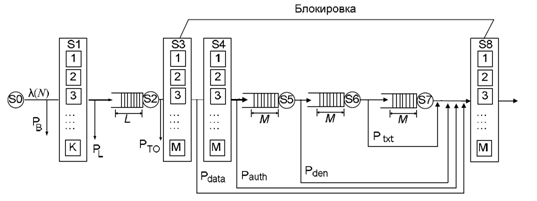
\includegraphics [scale=0.9] {net.jpg}
% %   \caption{Открытая сеть массового обслуживания, формализующая работу КХЭД} 
% %   \label{img:net}  
% % \end{figure}
% \begin{figure}[h]
%   \centering
%   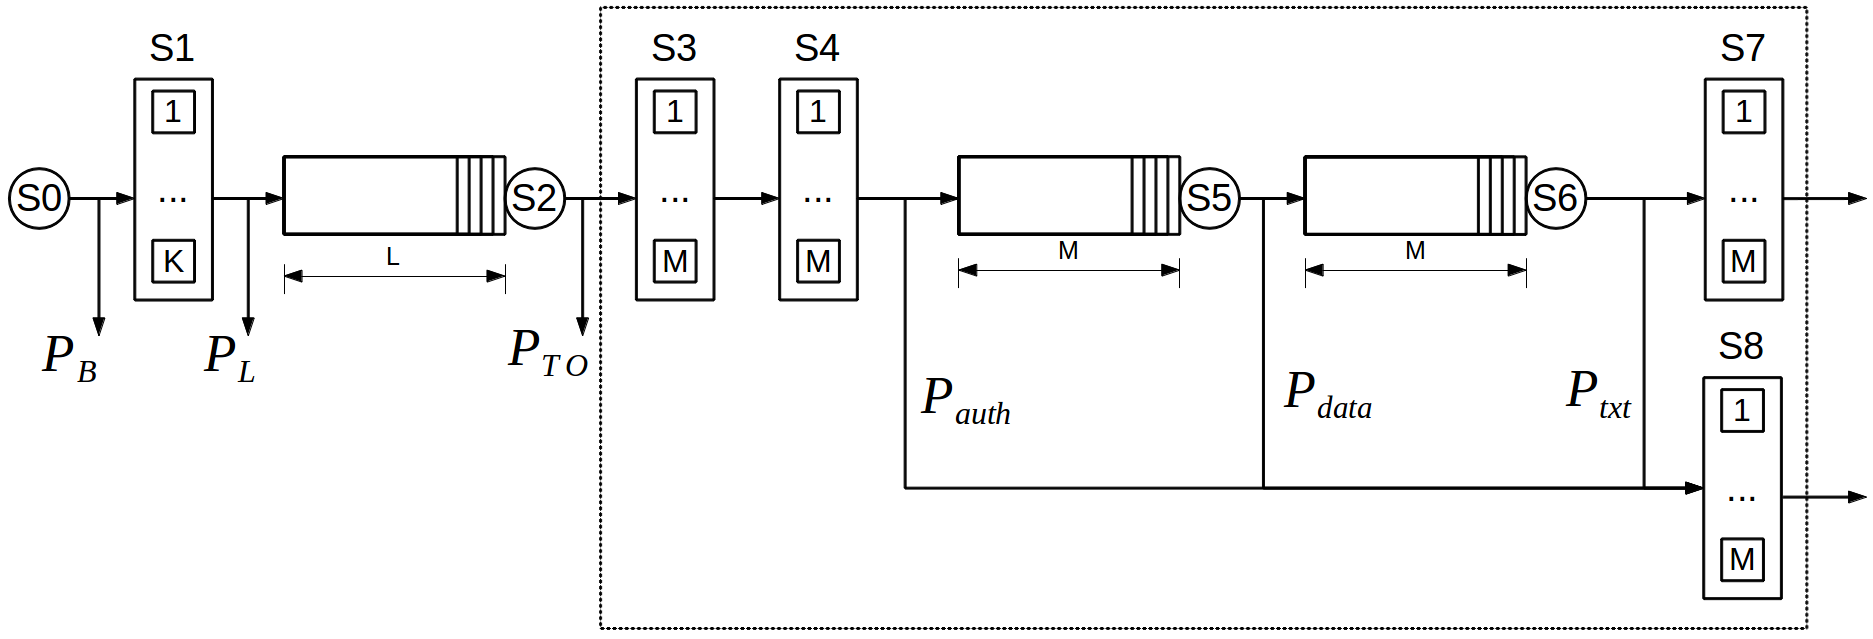
\includegraphics[width=1\textwidth]{net}
%   \caption{Открытая сеть массового обслуживания, формализующая работу КХЭД}
%   \label{img:net}
% \end{figure}

% $S0$ -- центр, формализующий входной поток сообщений пользователей.

% $S1$ -- центр, формализующий работу модуля TCP (транспортный уровень) операционной системы сервера приложений КХЭД на этапе установления соединения. $K$ – число обслуживающих каналов, очередь отсутствует. Если в момент поступления сообщения в центр все $K$ каналов заняты, то сообщение теряется, вероятность этого события равна $P_B$.

% $S2$ -- основной поток приложения сервера, извлекающего сообщения из очереди на установление соединения. Максимальная длина очереди $L$ к центру задается в серверном приложении. Если при поступлении сообщения все $L$ мест очереди заняты, то сообщение теряется с вероятностью $P_L$.

% $S3$ -- параллельные потоки сервера, обеспечивающие одновременное обслуживание соединений на этапе получения запросов по сети. При переполнении центра сообщения теряются с вероятностью $P_{TO}$.
% Центры $S1$, $S2$, $S3$ реализуют \underline{модуль установки соединения}.

% Центры $S3$ и $S8$ имеют по $M$ каналов обслуживания (потоков сервера) и при начале обслуживания сообщения в $i$-ом канале центра $S3$ он считается занятым до завершения обслуживания в $i$-ом канале центра $S8$. Таким образом, происходит блокировка каналов центров $S3$ и $S8$ и поэтому потерь сообщений из-за переполнения очереди к центрам $S5$, $S6$, $S7$ и занятости всех обслуживающих устройств центра $S4$ не происходит, т.к. больше чем $M$ сообщений в центрах $S4$, $S5$, $S6$, $S7$ быть не может.

% $S4$ -- \underline{модуль аутентификации} клиентов при обращении к КХЭД.

% $S5$ -- модуль \underline{проверки прав доступа} клиентов при обращении к КХЭД.

% В случае удачной аутентификации и проверки прав доступа клиента производится поиск электронного документа по запросу пользователя и выполнение операций по контролю целостности информации, проверке и простановки ЭЦП, шифрованию и дешифрованию. Для формализации процесса поиска и редактирования электронных документов выделены центры $S6$ и $S7$ соответственно.
% После того, как запрос пользователя выполнен, происходит передача ответа пользователю в многолинейном центре обслуживания $S8$.

% В соответствии с теоремой BCMP (Baskett, Chandy, Muntz, Palacios) мультипликативное свойство решения \ref{eq:equation1} для $P_(n_1,n_2,\ldots,n_R)$ сохраняется для СеМО, содержащих следующие виды узлов:
% \begin{itemize}
%   \item $M/M/m$ с дисциплиной обслуживания FCFS (First Came First Served -- первым поступил, первым обслужен);
%   \item $M/G/1$ с дисциплиной дисциплиной PS (Process Sharing -- разделение процессора);
%   \item $M/G/\infty$ с обслуживанием без ожидания (IS -- Immediately Serve);
%   \item $M/G/1$ с дисциплиной LCFS (Last Came First Served -- последним поступил, первым обслужен) с прерываниями.\cite{bib7}
% \end{itemize}

% В приведённой на рис. \ref{img:net} схеме представлены следующие узлы:
% \begin{itemize}
%   \item $S1, S3, S4, S8 - M/G/\infty$, IS;
%   \item $S2, S6, S7 - M/M/1$, FCFS;
%   \item $S5 - M/G/1$, PS.\cite{bib3}
% \end{itemize}

% Одной из важнейших задач СЭД является обнаружение ошибок редактора. Такие ошибки делятся соответственно на \textit{детектируемые} и \textit{недетектируемые}.
% Описанная на рис. \ref{img:net} СеМО обнаруживает следующие типы ошибок:
% \begin{itemize}
%   \item Неверное предоставление аутентификационных данных -- эта ошибка появляется с вероятностью $P_{data}$;
%   \item Отсутствие прав доступа к запрашиваемому документу -- с вероятностью $P_{auth}$;
%   \item Ошибка поиска -- с вероятностью $P_{den}$;
%   \item Ошибки во вносимых изменениях (напр., обращение к некорректным полям документа) -- с вероятностью $P_{txt}$.
% \end{itemize}

% Механизм обнаружения таких ошибок позволяет избежать выдачи заведомо неверного документа следующему редактору в схеме, представленной на рис. \ref{img:graph1}.

% С учётом вышеописанного, каждый из редакторов в схеме на рис. \ref{img:graph1} может быть представлен в виде автоматизированной системы, изображённой на рис. \ref{img:as}.

% \begin{figure}[h]
%   \centering
%   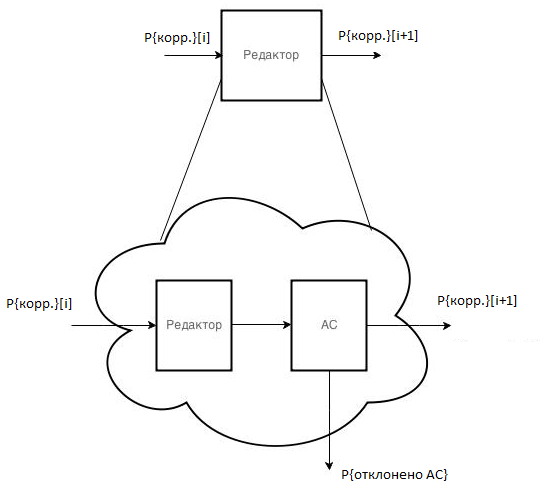
\includegraphics[width=1\textwidth]{as}
%   \caption{Схема узла СЭД с применением АС для обработки данных}
%   \label{img:as}
% \end{figure}

% В роли АС здесь выступает КХЭД, описанное на рис. \ref{img:net}. В случае обнаружения ошибок силами АС пользователю выдаётся сообщение об ошибке, т.е. фактически новое задание на редактирование. С учётом этого факта граф, представленный на рис. \ref{img:graph1}, преобразуется к виду:

% \begin{figure}[h]
%   \centering
%   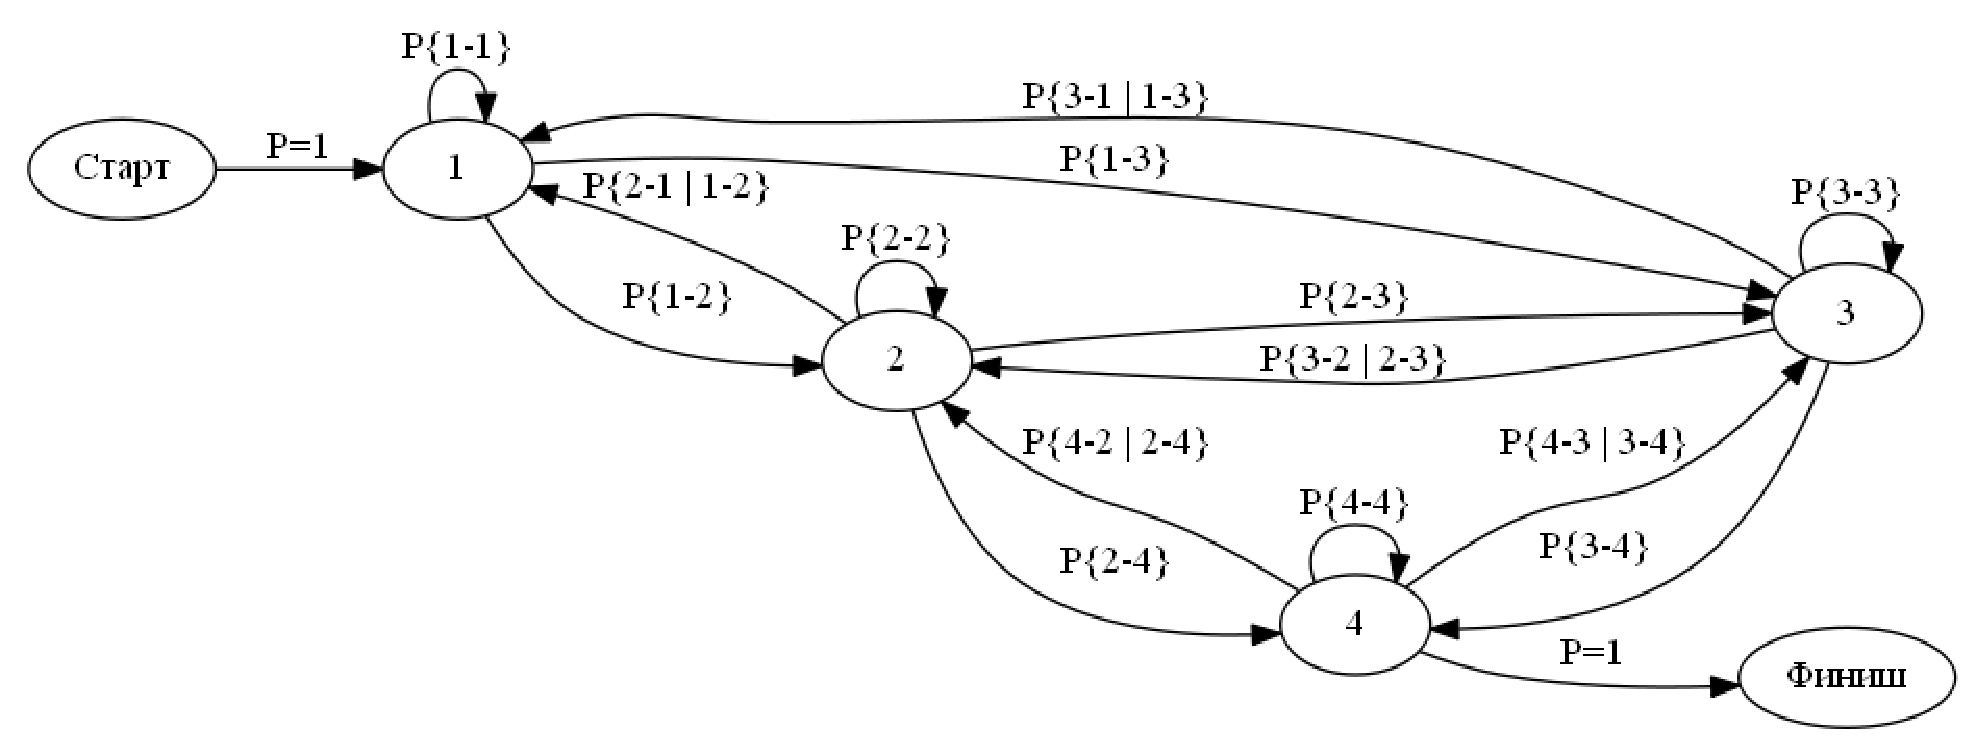
\includegraphics[width=1\textwidth]{graph2}
%   \caption{Документооборот с применением СЭД}
%   \label{img:graph2}
% \end{figure}

% \clearpage
% \newpage

% \subsection{Математическая постановка задачи} \label{sect1_3}

% \clearpage
% \newpage

% \subsection{Заключение} \label{sect1_3}

% В ходе прохождения практики были самостоятельно проработаны все материалы, данные руководителем практики, с целью повышения результативности работы, а также дальнейшего использования полученных знаний в подготовке дипломного проекта.

% Также были выполнено следующее:
% \begin{itemize}
%   \item произведено исследование состава системы электронного документооборота;
%   \item проанализирована структура конфиденциального хранилища электронных документов;
%   \item конфиденциальное хранилище электронных документов рассмотрено и описано с точки зрения теории массового обслуживания;
%   \item подготовлена математическая постановка задачи для дипломного проекта.
% \end{itemize}
% \clearpage